\xchapter{模拟器验证与瓶颈及热点分析实验}{Simulator Validation, Bottleneck and Hotspot Analysis Experiments}

\xsection{模拟器基本功能与精度验证}{Basic Functionality and Accuracy Validation}

本节通过可控微基准与硬件模拟平台对照，验证三项核心能力：多核之间通过片上网络进行同步、多核之间通过 DRAM 进行同步，以及单核下与 ZeBu 硬件模拟的总周期精度。片上网络同步实验与内存同步实验均在两档后端下分别运行以做对照。

\xsubsection{片上网络同步实验}{NoC Synchronization Experiment}

实验原理方面，本实验构造一个最小的双核、点对点（Peer-to-Peer，P2P）数据依赖场景，用于验证“消费者核心必须等到生产者数据到达后才能开始计算”的因果一致性。具体而言：第一个核心（Core\,0）作为生产者，先从片外存储器（DRAM）加载权重 \SI{32}{KB} 与输入特征 \SI{8}{KB}，接着进行 500 个模拟周期的计算，产生 \SI{128}{KB} 的输出并可供其他核心读取。第二个核心（Core\,1）作为消费者，需要先从 DRAM 加载自己的权重 \SI{64}{KB}，同时必须等待 Core\,0 产出的 \SI{128}{KB} 数据作为自己的输入特征，二者都就绪后再进行 300 周期计算，最后将结果写回 DRAM。若模拟器正确实现依赖传播，则 Core\,1 在加载阶段应一直等待，直到 Core\,0 的输出经核间通路到达后，才能结束加载、进入计算阶段。

实验过程上，硬件与负载配置如下。硬件配置：双核拓扑。NoC 与 DRAM 分别采用前文定义的 高保真后端（BookSim2 + Ramulator2，完整建模 DDR 时序与网络排队）与 简化后端（固定延迟、简化建模）各运行一次，以对比两种后端下核间依赖与访存延迟的叠加效果。运行负载：即上述“Core\,0 生产者、Core\,1 消费者”的两层调度，输入与权重规模如上。实验时对两种后端分别执行模拟，并开启状态记录。从模拟得到的状态时间线中读取每个核心在加载、计算、写回各阶段的起始与结束周期，以及各阶段持续时长，用于填表与绘图。

实验结果方面，表\ref{tab:mb1}给出两种后端下各核的状态转移时间点与阶段时长。

\begin{table}[H]
  \centering
  \caption{片上网络同步实验结果}
  \label{tab:mb1}
  \small
  \begin{tabular*}{\textwidth}{@{\extracolsep{\fill}}llrrr}
    \toprule
    后端 & 核/阶段 & 起始周期 & 结束周期 & 时长 \\
    \midrule
    \multirow{5}{*}{高保真后端} & Core\,0 LOADING  & 0    & 207  & 207 \\
                                    & Core\,0 COMPUTING & 207  & 707  & 500 \\
                                    & Core\,1 LOADING  & 0    & 2000 & 2000 \\
                                    & Core\,1 COMPUTING & 2000 & 2300 & 300 \\
                                    & Core\,1 WRITEBACK & 2300 & 2456 & 156 \\
    \cmidrule{2-5}
                                    & 总周期 & \multicolumn{3}{r}{2458} \\
    \midrule
    \multirow{5}{*}{简化后端} & Core\,0 LOADING  & 0   & 180 & 180 \\
                             & Core\,0 COMPUTING & 180 & 680 & 500 \\
                             & Core\,1 LOADING  & 0   & 938 & 938 \\
                             & Core\,1 COMPUTING & 938 & 1238 & 300 \\
                             & Core\,1 WRITEBACK & 1238 & 1402 & 164 \\
    \cmidrule{2-5}
                             & 总周期 & \multicolumn{3}{r}{1404} \\
    \bottomrule
  \end{tabular*}
\end{table}

图\ref{fig:c5_mb1_trace}根据高保真后端运行得到的状态转移踪迹绘制，横轴为模拟周期（Cycle），纵轴为两核（上方为 Core\,1，下方为 Core\,0），图中颜色表示各核所处状态：橙色为 LOADING，蓝色为 COMPUTING，红色为 WRITEBACK。该图直观展示两核的状态转移时间线：Core\,0 先完成 LOADING 与 COMPUTING，Core\,1 在长时间 LOADING（等待 Core\,0 的输出与 DRAM 响应）后才进入 COMPUTING 与 WRITEBACK，与表\ref{tab:mb1}一致。

\begin{figure}[H]
  \centering
  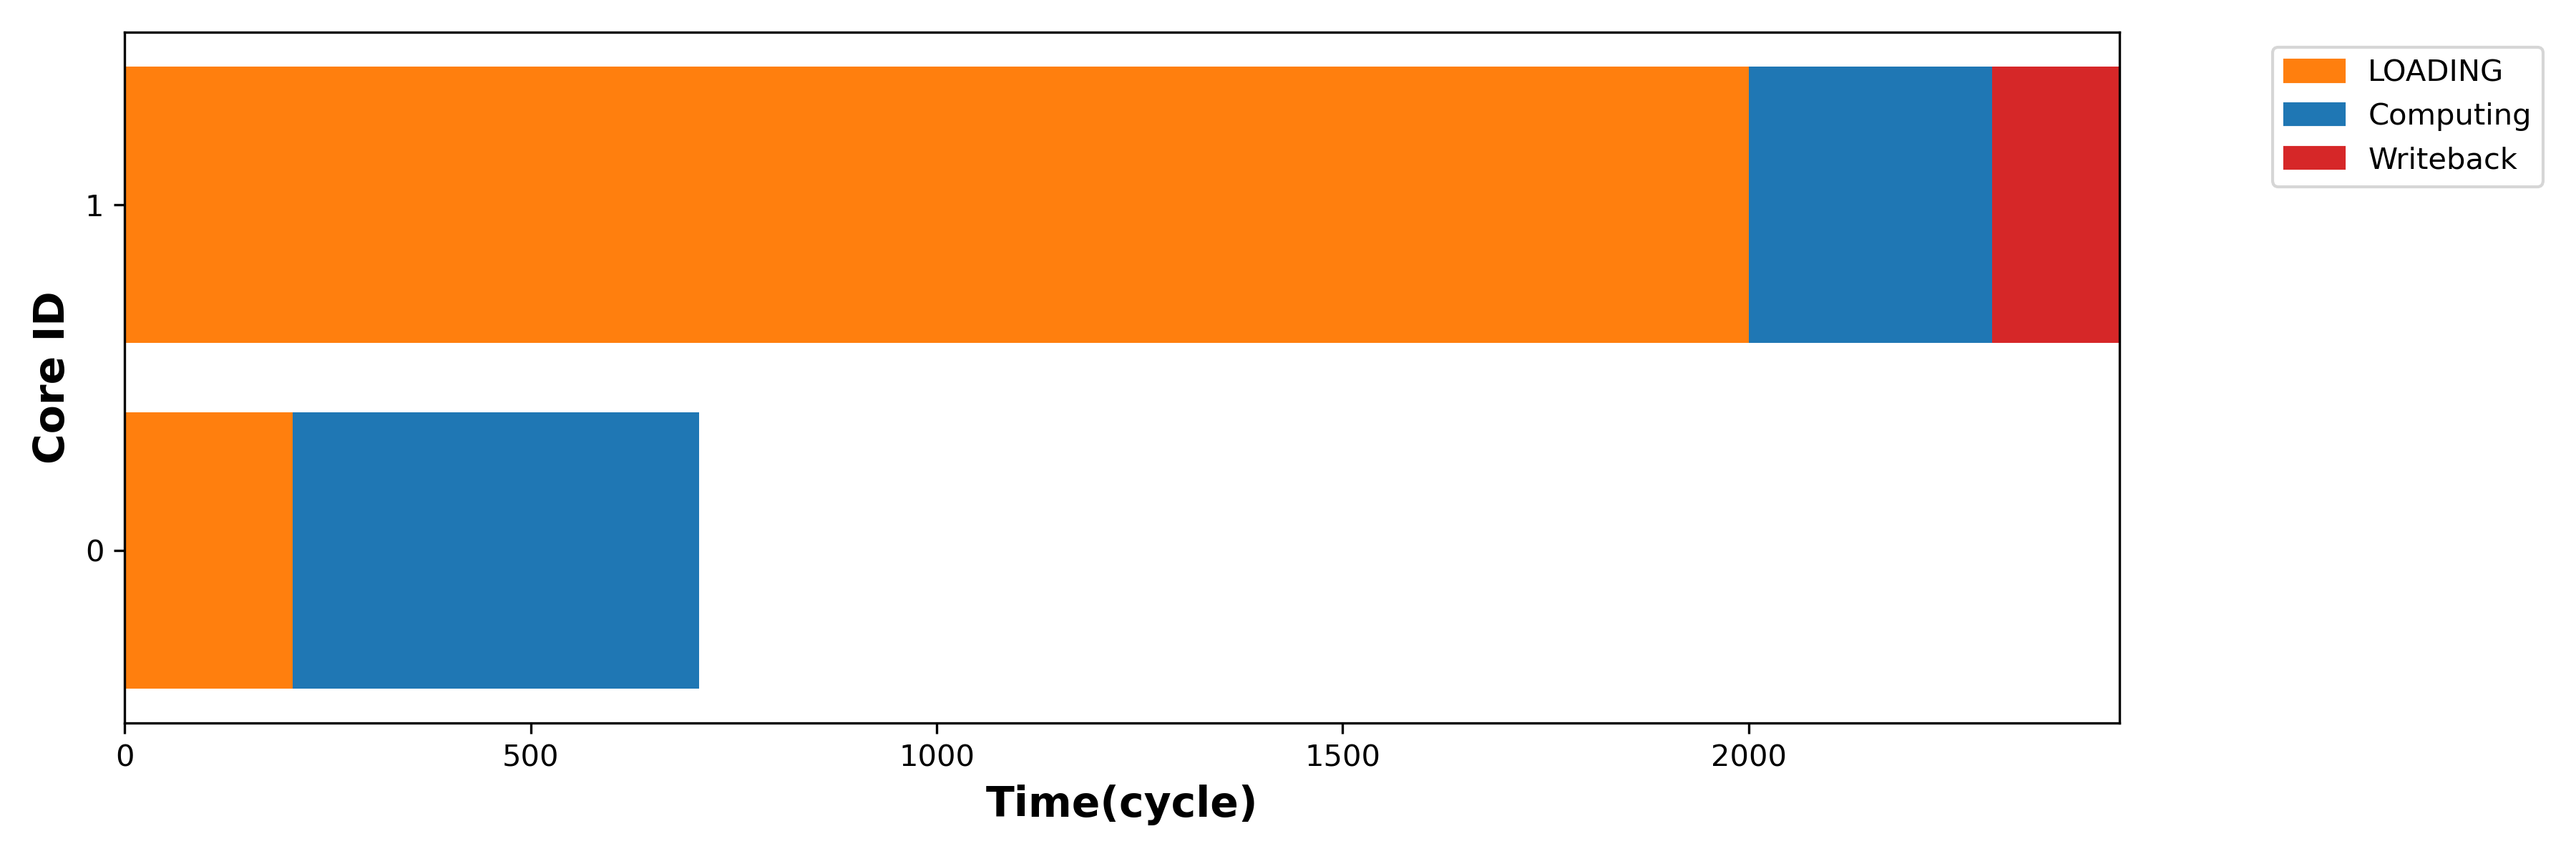
\includegraphics[width=0.78\linewidth]{Figures/c5_mb1_trace.png}
  \caption{片上网络同步实验高保真后端状态转移时间线}
  \label{fig:c5_mb1_trace}
\end{figure}

对结果的分析如下：（1）因果一致性验证通过。两种后端下，Core\,1 均在 Core\,0 完成计算（高保真后端下约 707 周期，简化后端下约 680 周期）之后才结束加载阶段、进入计算阶段（高保真后端下 Core\,1 加载约 2000 周期，简化后端下约 938 周期），说明依赖传播的因果约束被正确执行。模拟输出的状态记录也显示，Core\,1 在加载阶段明确标记为“等待来自 Core\,0 的 \SI{128}{KB} 数据”，与上述依赖关系一致。（2）计算时长一致。两种后端下 Core\,0 与 Core\,1 的计算阶段分别为 500 与 300 周期，与调度中设定的计算量完全吻合，验证了计算建模的正确性。（3）DRAM 后端影响访存阶段。高保真后端下 Core\,1 的 LOADING 阶段为 2000 周期，简化后端下仅为 938 周期。差异来自 Ramulator2 的 DDR4 时序约束（tRCD、tCL 等）使 DRAM 响应延迟更高，同时 Core\,1 还需等待 Core\,0 的计算及 NoC 传输完成，两者串行叠加导致 LOADING 时间显著拉长。（4）NoC 数据包一致。两种后端均产生 2 个 NoC 数据包（从 Core\,0 到 Core\,1 的请求与响应），验证了核间通信路径的正确性。

\xsubsection{内存同步实验}{Memory Synchronization Experiment}

实验原理方面，本实验在单核上执行两层串行计算，且两层所需的输入与权重全部来自片外存储器（DRAM），不涉及核间数据传递，用于验证：（1）单核、仅 DRAM 依赖时，不应产生任何 NoC 数据包。（2）简化后端与高保真后端两种后端在纯 DRAM 访存场景下的周期差异，量化 DDR 时序建模对访存阶段的影响。具体负载为：第一层从 DRAM 加载权重 \SI{32}{KB} 与输入特征 \SI{8}{KB}，计算 500 周期后向 DRAM 写回 \SI{128}{KB}。第二层从 DRAM 加载权重 \SI{64}{KB} 与输入特征 \SI{128}{KB}（即第一层写回的数据），计算 300 周期后向 DRAM 写回 \SI{32}{KB}。两层的计算量固定，差异仅体现在 DRAM 的加载与写回阶段上。

实验过程上，硬件配置为单核拓扑，NoC 与 DRAM 仍分别采用 高保真后端与 简化后端各运行一次。运行负载即上述“两层、仅 DRAM 依赖”的调度，无核间通信。对两种后端分别执行模拟并记录状态时间线，从时间线中读取每一层在加载、计算、写回各阶段的起止周期与时长，用于填表与对比。

实验结果方面，两种后端下各层的执行时间线见表\ref{tab:mb2}。

对结果的分析如下：（1）NoC 数据包为 0。两种后端下均无 NoC 流量（DRAM 直连核，未经过 NoC），验证了单核 DRAM-only 场景下通信路径的正确性。（2）计算时长一致。Layer1 与 Layer2 的 COMPUTING 阶段在两种后端下分别为 500 与 300 周期，与调度中给定的计算周期一致。（3）DRAM 模型差异集中在访存阶段。高保真后端下，Layer1 的 WRITEBACK 为 651 周期（简化后端 356，增幅 83\%），Layer2 的 LOADING 为 853 周期（简化后端 484，增幅 76\%）。这反映了 Ramulator2 的 DDR4 时序（行激活、列读取、Bank 冲突、请求排队）对大块数据传输的影响：Layer1 写回 \SI{128}{KB}、Layer2 加载 \SI{192}{KB}（64+128），数据量越大时 DDR 时序约束越显著。（4）总周期差异。高保真后端总周期 2685，简化后端为 1987，高保真后端高出 35\%。差异完全来自 DRAM 访存阶段，计算阶段无差异。后续 ZeBu 对比实验统一采用高保真后端，以在包含完整 DDR 时序建模的条件下评估模拟器的端到端精度。

\begin{table}[H]
  \centering
  \caption{内存同步实验结果}
  \label{tab:mb2}
  \small
  \begin{tabular*}{\textwidth}{@{\extracolsep{\fill}}llrrr}
    \toprule
    后端 & 层/阶段 & 起始周期 & 结束周期 & 时长 \\
    \midrule
    \multirow{7}{*}{高保真后端} & Layer1 LOADING    & 0    & 207  & 207 \\
                                    & Layer1 COMPUTING  & 207  & 707  & 500 \\
                                    & Layer1 WRITEBACK  & 707  & 1358 & 651 \\
                                    & Layer2 LOADING    & 1359 & 2212 & 853 \\
                                    & Layer2 COMPUTING  & 2212 & 2512 & 300 \\
                                    & Layer2 WRITEBACK  & 2512 & 2683 & 171 \\
    \cmidrule{2-5}
                                    & 总周期 & \multicolumn{3}{r}{2685} \\
    \midrule
    \multirow{7}{*}{简化后端} & Layer1 LOADING    & 0    & 180  & 180 \\
                             & Layer1 COMPUTING  & 180  & 680  & 500 \\
                             & Layer1 WRITEBACK  & 680  & 1036 & 356 \\
                             & Layer2 LOADING    & 1037 & 1521 & 484 \\
                             & Layer2 COMPUTING  & 1521 & 1821 & 300 \\
                             & Layer2 WRITEBACK  & 1821 & 1985 & 164 \\
    \cmidrule{2-5}
                             & 总周期 & \multicolumn{3}{r}{1987} \\
    \bottomrule
  \end{tabular*}
\end{table}

片上网络同步实验与内存同步实验小结。两个微基准验证了模拟器三项基本能力：核间依赖因果一致性（片上网络同步实验）、DRAM 闭环正确性（内存同步实验）、以及简化后端/高保真后端在计算阶段完全一致而在访存阶段体现 DDR 时序差异。这为后续统一采用 高保真后端进行 ZeBu 精度校验与多核设计空间探索奠定了基础。

\xsubsection{模拟器精度验证实验}{Simulator Accuracy Validation Experiment}
\label{subsec:c5_zebu}

实验原理方面，Synopsys ZeBu硬件模拟平台在单核配置下执行与本模拟器相同的调度IR所生成的汇编指令，并通过硬件踪迹记录每条指令的执行区间$[\mathit{start},\mathit{end}]$。以ZeBu全程序总周期（$\max(\mathit{end})$）作为基准，与本模拟器的Total cycles对比，相对误差定义为$(\text{模拟器}-\text{ZeBu})/\text{ZeBu}\times 100\%$。为使精度评估涵盖完整的系统级时序（包括 DDR 行列时序与请求排队），本实验采用高保真后端（BookSim2 + Ramulator2）与 ZeBu 硬件模拟对照。

实验过程上，ZeBu 侧的总周期取自 Gemini-Compiler-IR 项目发布的单核预跑结果（与第二章所述一致）。本实验在模拟器一侧采用单核、高保真后端配置（BookSim2 + Ramulator2），选取 ResNet34 与 ResNet50 在批大小 1 与 4 下的调度结果分别运行模拟并记录总周期，与上述 ZeBu 参考周期逐项对比。

实验结果方面，表\ref{tab:zebu_validation}给出上述四种配置下模拟器与 ZeBu 的总周期及相对误差。

\begin{table}[H]
  \centering
  \caption{与 ZeBu 硬件模拟的总周期对比表}
  \label{tab:zebu_validation}
  \small
  \begin{tabular*}{\textwidth}{@{\extracolsep{\fill}}lrrrr}
    \toprule
    模型 & 批大小 & ZeBu周期 & 模拟器周期 & 相对误差（\%） \\
    \midrule
    ResNet34 & 1  & 1,922,067 & 1,890,695 & $-$1.63 \\
    ResNet34 & 4  & 4,280,215 & 4,501,725 & +5.18 \\
    ResNet50 & 1  & 2,545,655 & 2,432,592 & $-$4.44 \\
    ResNet50 & 4  & 5,470,662 & 5,653,354 & +3.34 \\
    \bottomrule
  \end{tabular*}
\end{table}

对结果的分析如下：（1）误差均在 $\pm$5.2\% 以内。4 种配置的相对误差范围为 $-$4.44\% 至 +5.18\%，说明在包含完整 DRAM 时序建模的条件下，模拟器与 ZeBu 硬件模拟在总周期上吻合良好。（2）正负偏差并存，无系统性偏移。批大小为 1 时模拟器周期略低于 ZeBu（$-$1.63\%、$-$4.44\%），批大小为 4 时略高（+5.18\%、+3.34\%），偏差方向与批大小有关：批较小时 Ramulator2 的 DDR 时序对小规模访存的建模与 ZeBu 存在微小差异，批增大后工作负载级阶段划分与 ZeBu 指令级执行在访存重叠上的建模粒度差异被放大。（3）趋势一致。随批大小从 1 增至 4，两个模型的总周期均近似线性增长（ResNet34 由 1.89M 增至 4.50M，对应 ZeBu 由 1.92M 增至 4.28M。ResNet50 由 2.43M 增至 5.65M，对应 ZeBu 由 2.55M 增至 5.47M），趋势一致。

\xsubsection{实验结论}{Experimental Conclusions}

综合片上网络同步实验、内存同步实验与模拟器精度验证实验三组实验，本节得到以下结论。片上网络同步实验验证了模拟器在双核点对点依赖下的因果一致性，状态机在等待数据后进入计算的行为符合预期。内存同步实验通过 简化后端与高保真后端在不同并发度下的对比，印证了可插拔后端在“快速校验”与“高保真评估”间的不同定位。在单核、调度一致、统一采用 高保真后端（BookSim2 + Ramulator2，包含完整 DDR 行列时序与请求排队）的配置下，本模拟器与 ZeBu 硬件模拟平台在 4 种 ResNet 配置上的总周期相对误差均控制在 $\pm$5.2\% 以内，验证了端到端时序模型的准确性。三组实验共同表明，本模拟器具备可信的建模能力，为后续多核瓶颈分析与设计空间探索提供了可靠基础。

\xsection{性能瓶颈优化实验}{Performance Bottleneck Optimization Experiments}

在 5.1 节验证了模拟器的核间因果一致性、DRAM 闭环正确性与端到端总周期精度的基础上，本节围绕"识别瓶颈—解释瓶颈—消除瓶颈"这一主线，基于本文模拟器对神经网络芯片在真实 DNN 负载下的性能瓶颈展开系统性分析与逐级优化。本节由两组前后衔接的实验与一段整体结论构成：5.2.1 节先在单核配置下对 ResNet34 与 ResNet50 进行端到端阶段占比分解与按核可视化，建立"计算占比/访存占比/NoC 背压占比"的可解释归因框架；5.2.2 节将分析对象扩展至 4 核多核配置，在同一 ResNet50 负载上以 DDR4 单通道为基线，沿"DDR4 → HBM → HBM + 宽 SRAM 端口"的递进路线进行三轮模拟，每一轮的硬件改动均由前一轮模拟暴露的瓶颈结论触发，从而在迭代中暴露并依次消除片外带宽与片上供数两类瓶颈；5.2.3 节在前两组实验之上汇总跨单核/多核场景的整体结论，给出对未来神经网络芯片在算力—存储平衡上的设计启示。需要说明的是，5.2.1 与 5.2.2 虽然在硬件配置与负载规模上有所差异，但分解口径完全一致，由此保证了两组实验结论可在同一框架下相互对照与递进汇总。

\xsubsection{单核性能瓶颈分析实验}{Single-core Performance Bottleneck Analysis Experiment}
\label{subsec:c5_singlecore}

本小节选取 ResNet34 与 ResNet50 两类负载，以调度器生成 IR 驱动模拟，通过端到端阶段占比分解与按核可视化，实现对单核性能瓶颈的可解释归因。

实验原理方面，端到端执行时间可拆分为“计算占用”与“等待占用”。本文采用可复现的近似拆分如下：
\begin{equation}
  T_\text{COMPUTING} = \sum_c C^\text{comp}_c\label{eqn:c5:bottleneck_compute}
\end{equation}
\begin{equation}
  T_\text{NoC\_Stall} = \sum_c C^\text{nocstall}_c\label{eqn:c5:bottleneck_nocstall}
\end{equation}
\begin{equation}
  T_\text{Mem\_Stall} \approx \sum_c C^\text{wb}_c + \sum_c C^\text{load}_c - \sum_c C^\text{nocstall}_c\label{eqn:c5:bottleneck_memstall}
\end{equation}
式中：$T_\text{COMPUTING}$ 为端到端总计算时间，由各核 COMPUTING 阶段周期 $C^\text{comp}_c$ 求和得到。$T_\text{NoC\_Stall}$ 为端到端 NoC 背压时间，由各核因网络背压而停滞的周期 $C^\text{nocstall}_c$ 求和得到。$T_\text{Mem\_Stall}$ 为端到端访存相关等待时间，近似为各核 WRITEBACK 阶段周期 $C^\text{wb}_c$ 与 LOADING 阶段周期 $C^\text{load}_c$ 之和减去已计入的 NoC 背压。下标 $c$ 为核心索引。单核场景下无核间通信，故 $T_\text{NoC\_Stall}=0$，瓶颈主要体现在计算与访存（DRAM 读/写）的占比上。

实验过程上，采用 Gemini-Compiler-IR 中 ResNet34 与 ResNet50 的调度结果（与第\,\ref{subsec:c5_zebu}\,节 ZeBu 对比实验同源）作为输入，在单核、简化后端配置下运行模拟器。模拟结束后，从输出的“每核统计”中读取每个核心在加载、计算、写回以及因网络背压而停滞的周期数，按上式汇总为总计算时间 $T_\text{COMPUTING}$、NoC 背压时间 $T_\text{NoC\_Stall}$ 与访存相关等待时间 $T_\text{Mem\_Stall}$，并计算三者占总执行时间的百分比。单核下无核间通信，NoC 背压恒为 0，瓶颈主要体现在计算与访存的占比上。表中给出批大小 1的分解结果。

实验结果方面，表\ref{tab:bottleneck}给出 ResNet34 与 ResNet50 在批大小 1、单核下的总周期及 $T_\text{COMPUTING}$、$T_{\mathrm{NoC}}$、$T_{\mathrm{Mem}}$ 的周期与占比，本实验中 $T_{\mathrm{NoC}}=0$。

\begin{table}[H]
  \centering
  \caption{真实负载端到端瓶颈分解表}
  \label{tab:bottleneck}
  \small
  \begin{tabular*}{\textwidth}{@{\extracolsep{\fill}}lrrcrccc}
    \toprule
    模型 & 总周期 & $T_\text{COMPUTING}$ & $T_{\mathrm{NoC}}$ & $T_{\mathrm{Mem}}$ & 计算\% & NoC\% & 访存\% \\
    \midrule
    ResNet34 & 1,890,695 & 1,530,664 & 0 & 359,888 & 81.0 & 0.0 & 19.0 \\
    ResNet50 & 2,432,592 & 1,863,694 & 0 & 568,717 & 76.6 & 0.0 & 23.4 \\
    \bottomrule
  \end{tabular*}
\end{table}

对结果的分析如下：（1）NoC 背压为 0。单核下无核间通信，$T_{\mathrm{NoC}}=0$，与预期一致。（2）计算为主导瓶颈。ResNet34 与 ResNet50 的计算占比分别为 81.0\% 与 76.6\%，说明在单核配置下端到端时间主要由计算阶段占据，与两类 CNN 的计算密度相符。（3）访存占比随模型加深而上升。ResNet50 的访存占比（23.4\%）高于 ResNet34（19.0\%），与 ResNet50 层数更多、中间激活与权重量更大、DRAM 读写的相对占比升高一致。多核映射下核间依赖与 NoC 竞争将引入非零 $T_\text{NoC\_Stall}$，届时可用同一分解框架区分计算与通信/访存瓶颈。

\begin{figure}[H]
  \centering
  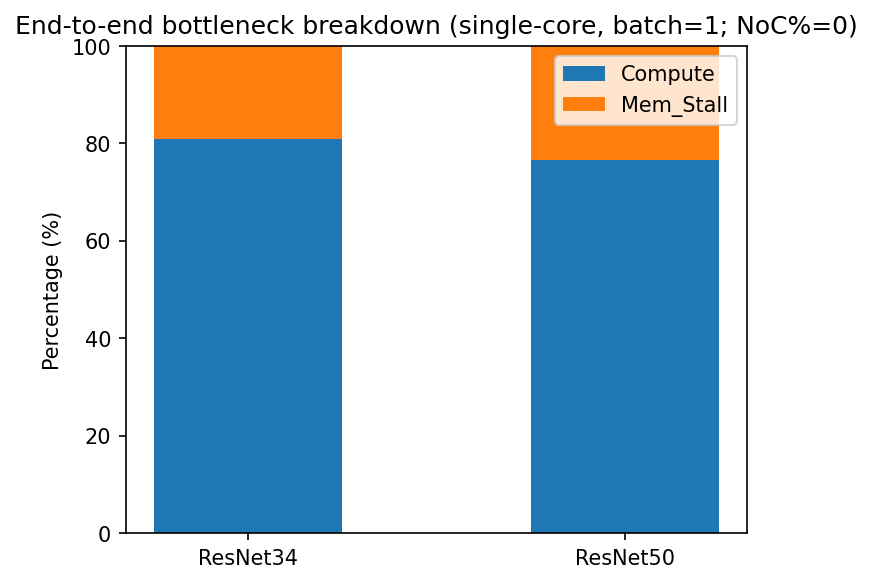
\includegraphics[width=0.65\linewidth]{Figures/c5_breakdown.png}
  \caption{端到端瓶颈占比图}
  \label{fig:c5_breakdown}
\end{figure}

在上述宏观分解之上，本小节进一步从按核维度给出可视化呈现，作为对宏观占比的空间补充。该可视化不引入新的模拟运行，而是基于上文单核 ResNet 统计与 5.1 节片上网络同步实验状态轨迹，扩展出"按核、按阶段"的形式：在双核微基准上以各核各阶段占该核活跃时间的比例热力图呈现，在单核真实负载上以与分解口径一致的阶段占比堆叠条呈现。

"热点核"在本文中定义为：在给定维度（如总周期占比、计算周期占比、访存等待周期占比或 NoC 背压周期占比）上显著高于其他核心的核。模拟器在运行时可记录每个核心在每一模拟周期内所处的状态（加载、计算、写回或停滞），形成按核、按时间排列的状态时间线。据此可统计各核在各阶段的累计周期数（即上文单核统计的推广），进而识别计算或等待时间最长的若干核心。对于单核 ResNet，本节采用与表\ref{tab:bottleneck}一致的阶段占比堆叠条，与上文分解口径严格对照；对双核场景则复用 5.1 节中的片上网络同步实验状态轨迹，绘制各核各阶段占该核活跃时间的比例热力图，以演示"按核、按阶段"分解在多核情形下的可行性。

可视化数据来源与结果如下：（1）双核基准：复用 5.1 节片上网络同步实验在简化后端下的双核点对点依赖负载状态轨迹，由各核工作负载的加载、计算、写回周期按核归一化，得到各阶段占该核活跃时间的比例，绘制热点热力图（图\,\ref{fig:c5_hot_cores}）。（2）单核真实负载（ResNet34/50）：直接复用上文批大小 1、单核的统计结果，将 $T_\text{COMPUTING}$ 与 $T_\text{Mem\_Stall}$ 占总时间的比例以堆叠条呈现，与表\ref{tab:bottleneck} 及图\,\ref{fig:c5_breakdown} 一致。

结果分析方面，图\,\ref{fig:c5_hot_cores} 表明，在片上网络同步实验中 Core\,1 的加载阶段占该核活跃时间的比例显著高于 Core\,0，与 consumer 需同时等待 DRAM 与 Core\,0 数据的设定一致。计算阶段 Core\,0 占比更高，体现生产者核以计算为主、消费者核以等待与写回为主的分工。与 5.1 节表\ref{tab:mb1} 及因果一致性结论一致，Core\,0 先完成加载与计算，Core\,1 在长时间加载后方进入计算与写回。图\,\ref{fig:c5_breakdown} 与表\ref{tab:bottleneck} 一致地表明，单核 ResNet 端到端时间仍以计算为主、访存相关等待次之，ResNet50 的访存占比高于 ResNet34，单核真实负载上的阶段占比条与上文宏观分解一致。

\begin{figure}[H]
  \centering
  
\includegraphics[width=0.88\linewidth]{Figures/c5_522_hotspot_mb1.png}
  \caption{片上网络同步实验双核各阶段占该核活跃时间的比例热力图}
  \label{fig:c5_hot_cores}
\end{figure}

综上，单核场景下 ResNet34 / ResNet50 的端到端时间以计算为主导（占比约 77\%--81\%）、访存次之（19\%--23\%）、NoC 背压恒为 0，访存占比随模型加深而上升；按核可视化进一步揭示了生产者—消费者分工下的核间负载差异。本小节构建的"分解口径 + 按核可视化"框架既给出全局占比，也给出按核分布，将作为后续 5.2.2 节多核存储瓶颈定位与逐级优化实验的统一归因工具。

\xsubsection{多核存储瓶颈定位与逐级优化实验}{Multi-core Memory Bottleneck Identification and Iterative Optimization Experiment}
\label{subsec:c5_multicore}

5.2.1 节在单核配置下建立了端到端瓶颈分解与按核可视化的归因框架。本小节将分析对象扩展到多核（4 核）场景，使用高保真后端（BookSim2 + Ramulator2）运行真实 DNN 负载，沿"DDR4 → HBM → HBM + 宽 SRAM 端口"的递进路线进行三轮模拟，每一轮的硬件改动均由前一轮模拟暴露的瓶颈结论触发，最终在迭代中依次消除片外带宽与片上供数两类瓶颈。本小节后续所有图表均共享同一组实验设置：负载为 ResNet50、批大小为 1、4 核拓扑、高保真后端，三组 DRAM/SRAM 配置依次为 DDR4 单通道基线、HBM 四通道优化、以及 HBM 四通道 + \SI{1024}{B/cycle} 宽 SRAM 端口。后续 caption 中不再重复这些公共参数。

本小节的实验设置围绕三个目标依次推进：先构造一个存储受限的多核基线配置，使 DRAM 带宽成为性能瓶颈，在甘特图上直观表现为加载阶段占据大部分时间；继而将 DRAM 技术从 DDR4 升级为 HBM（高带宽存储器），展示带宽升级对端到端性能的改善，以此验证模拟器能正确反映 DRAM 子系统差异；最后在 HBM 升级暴露出片上 SRAM 写端口瓶颈后，进一步加宽 SRAM 端口，观察三阶段是否趋于平衡。

负载与 IR 生成  采用 ResNet50 网络，批大小为 1，通过 Gemini 编译器的 4 核映射模式生成调度 IR。IR 共含 288 个工作负载（每核 72 个），涉及约 \SI{90}{MB} 的 DRAM 读取与 288 次 DRAM 写回，涵盖了 ResNet50 全部卷积、池化与全连接层。

硬件配置上，两组配置共享相同的核心微架构（MAC 256、Vector 64、SRAM \SI{16}{MB}、核频 \SI{25}{MHz}）与 NoC 拓扑（4 核 Mesh，BookSim2 后端），差异仅在 DRAM 子系统：

\begin{table}[H]
  \centering
  \caption{多核瓶颈分析实验的两组 DRAM 配置表}
  \label{tab:c5_dram_configs}
  \small
  \begin{tabular*}{\textwidth}{@{\extracolsep{\fill}}lcc}
    \toprule
    参数 & DDR4 基线 & HBM 优化 \\
    \midrule
    DRAM 标准      & DDR4-2400R  & HBM-2Gbps \\
    通道数         & 1           & 4 \\
    Rank 数        & 1           & 1 \\
    峰值带宽       & \SI{19.2}{GB/s}  & \SI{128.0}{GB/s} \\
    等效带宽/核周期 & \SI{768}{B/cycle} & \SI{5120}{B/cycle} \\
    \bottomrule
  \end{tabular*}
\end{table}

DDR4 基线采用单通道以模拟带宽受限场景（峰值 \SI{19.2}{GB/s}），HBM 优化采用 4 通道 HBM（峰值 \SI{128.0}{GB/s}），峰值带宽提升约 6.7 倍。两组均使用 Ramulator2 后端，具备 DDR 行列时序、Bank 冲突与请求排队的全真建模。受行/Bank 冲突与 FR-FCFS 调度约束，实测有效带宽通常显著低于上述峰值，在 ResNet50 的 DRAM 访问模式下尤为明显，因此 DDR4 单通道仍会构成显著的访存瓶颈。

作为递进式优化的起点，第一轮模拟先在 DDR4 单通道配置下运行，目的是建立带宽受限的初始基线并据此定位首个性能瓶颈，为下一轮的硬件改动提供依据。表\ref{tab:c5_baseline_stats}给出 DDR4 基线配置下的模拟统计结果。

\begin{table}[H]
  \centering
  \caption{DDR4 基线模拟每核统计表}
  \label{tab:c5_baseline_stats}
  \small
  \begin{tabular*}{\textwidth}{@{\extracolsep{\fill}}crrrrc}
    \toprule
    核 & IDLE & LOADING & COMPUTING & WRITEBACK & Workloads \\
    \midrule
    0  & 0      & 140,680  & 22,352  & 64,537  & 72 \\
    1  & 0      & 153,077  & 22,352  & 58,929  & 72 \\
    2  & 0      & 144,515  & 22,352  & 66,362  & 72 \\
    3  & 0      & 153,799  & 22,352  & 62,381  & 72 \\
    \midrule
    总计/最大 & --- & 592,071 & 89,408 & 252,209 & 288 \\
    \bottomrule
  \end{tabular*}
\end{table}

总周期为 238,803。各核加载阶段占活跃时间的 60\%--65\%，计算阶段仅 9\%--10\%，写回阶段约 26\%--28\%。LOADING\allowbreak /COMPUTING \allowbreak 总比值达 6.6，表明系统处于严重的存储受限状态。图\ref{fig:c5_hotspot_ddr4}以热力图形式展示了各核各阶段占活跃时间的比例，LOADING 列颜色最深，直观反映 DRAM 带宽瓶颈。

\begin{figure}[H]
  \centering
  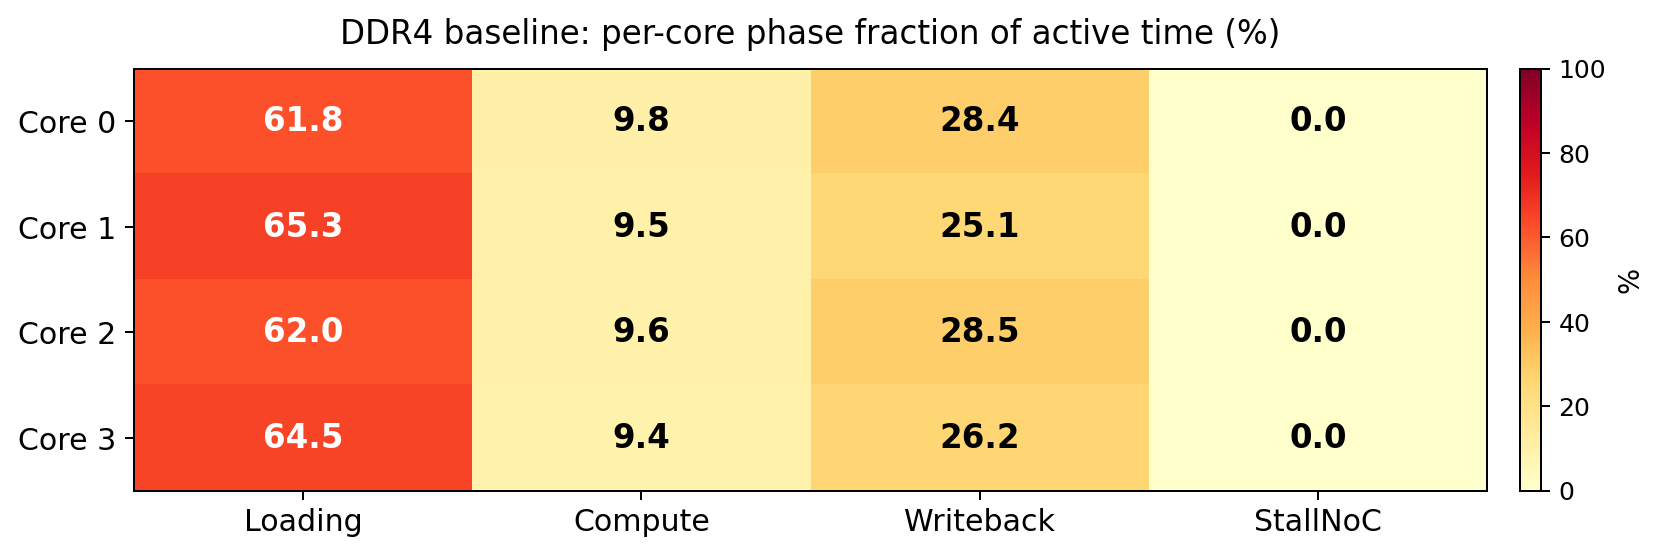
\includegraphics[width=0.88\linewidth]{Figures/c5_hotspot_ddr4_baseline.png}
  \caption{DDR4 基线各核阶段占比热力图}
  \label{fig:c5_hotspot_ddr4}
\end{figure}

图\ref{fig:c5_gantt_ddr4}给出 DDR4 基线的甘特图，实验条件为 4 核网格、ResNet50、批 1，颜色含义为橙色表示加载阶段（含 DRAM 读取与核间等待）、蓝色表示计算、红色表示写回。可见 4 核的加载段（橙色，含 DRAM 等待与核间等待子段）占据绝大部分时间线，计算段（蓝色）极为狭窄，直观展示了带宽瓶颈。

\begin{figure}[H]
  \centering
  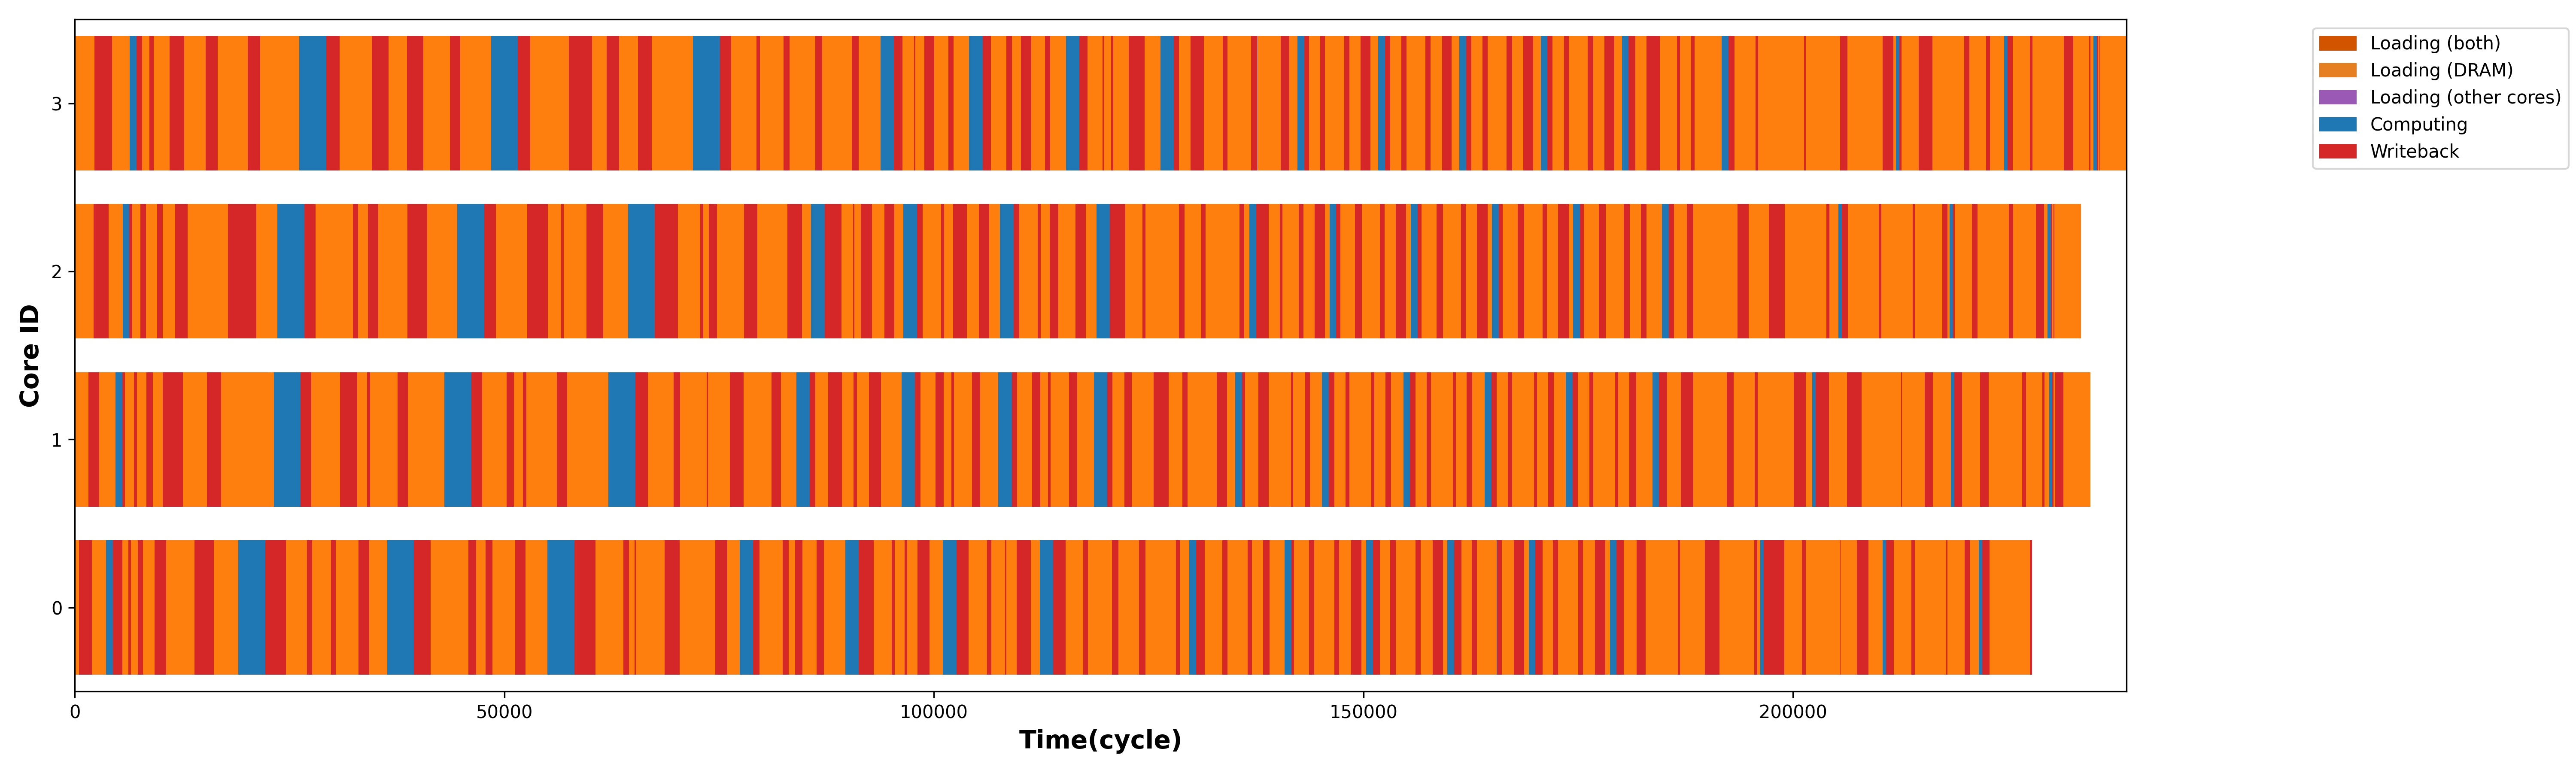
\includegraphics[width=\linewidth]{Figures/c5_gantt_ddr4_baseline.png}
  \caption{DDR4 基线甘特图}
  \label{fig:c5_gantt_ddr4}
\end{figure}

第一轮模拟将瓶颈定位在 DDR4 单通道的 DRAM 带宽侧，第二轮即针对该瓶颈进行硬件改动，将 DRAM 从 DDR4 单通道替换为 HBM 四通道，使峰值带宽从 \SI{19.2}{GB/s} 提升至 \SI{128.0}{GB/s}，其余配置保持不变，重新运行模拟以观察瓶颈是否消除或迁移，结果见表\ref{tab:c5_hbm_stats}。

\begin{table}[H]
  \centering
  \caption{HBM 优化模拟每核统计表}
  \label{tab:c5_hbm_stats}
  \small
  \begin{tabular*}{\textwidth}{@{\extracolsep{\fill}}crrrrc}
    \toprule
    核 & IDLE & LOADING & COMPUTING & WRITEBACK & Workloads \\
    \midrule
    0  & 0      & 84,488  & 22,352  & 18,092  & 72 \\
    1  & 0      & 102,664 & 22,352  & 18,713  & 72 \\
    2  & 0      & 85,616  & 22,352  & 18,093  & 72 \\
    3  & 0      & 97,415  & 22,352  & 18,533  & 72 \\
    \midrule
    总计/最大 & --- & 370,183 & 89,408 & 73,431 & 288 \\
    \bottomrule
  \end{tabular*}
\end{table}

总周期降至 144,000。LOADING/COMPUTING 比值从 6.6 降至 4.1，WRITEBACK 总周期从 252,209 降至 73,431（降幅 70.9\%）。图\ref{fig:c5_hotspot_hbm}的热力图显示，LOADING 占比仍在 67\%--71\%（因 SRAM 端口瓶颈），但 WRITEBACK 从 25\%--28\% 降至 13\%--15\%，COMPUTING 从 9\%--10\% 升至 16\%--18\%。

\begin{figure}[H]
  \centering
  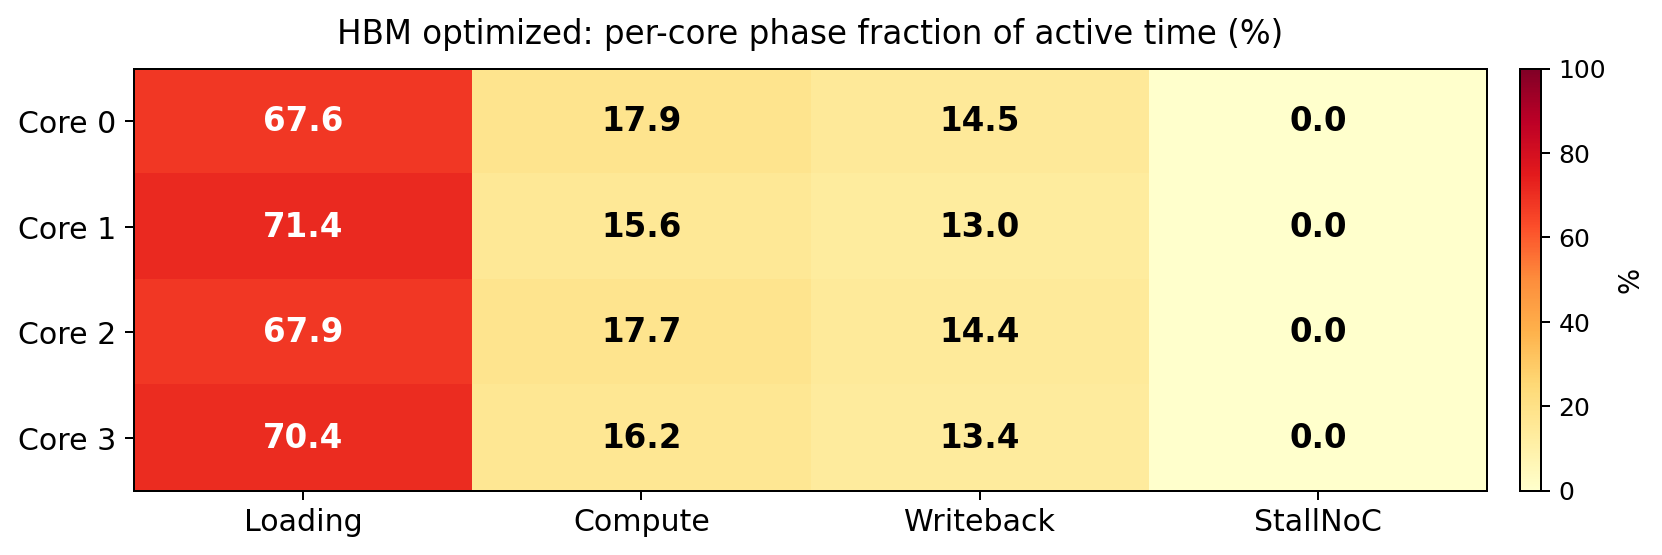
\includegraphics[width=\linewidth]{Figures/c5_hotspot_hbm_optimized.png}
  \caption{HBM 优化各核阶段占比热力图}
  \label{fig:c5_hotspot_hbm}
\end{figure}

图\ref{fig:c5_gantt_hbm}为 HBM 优化甘特图，可见写回段（红色）显著收窄，加载段虽仍为主导但已明显缩短。

\begin{figure}[H]
  \centering
  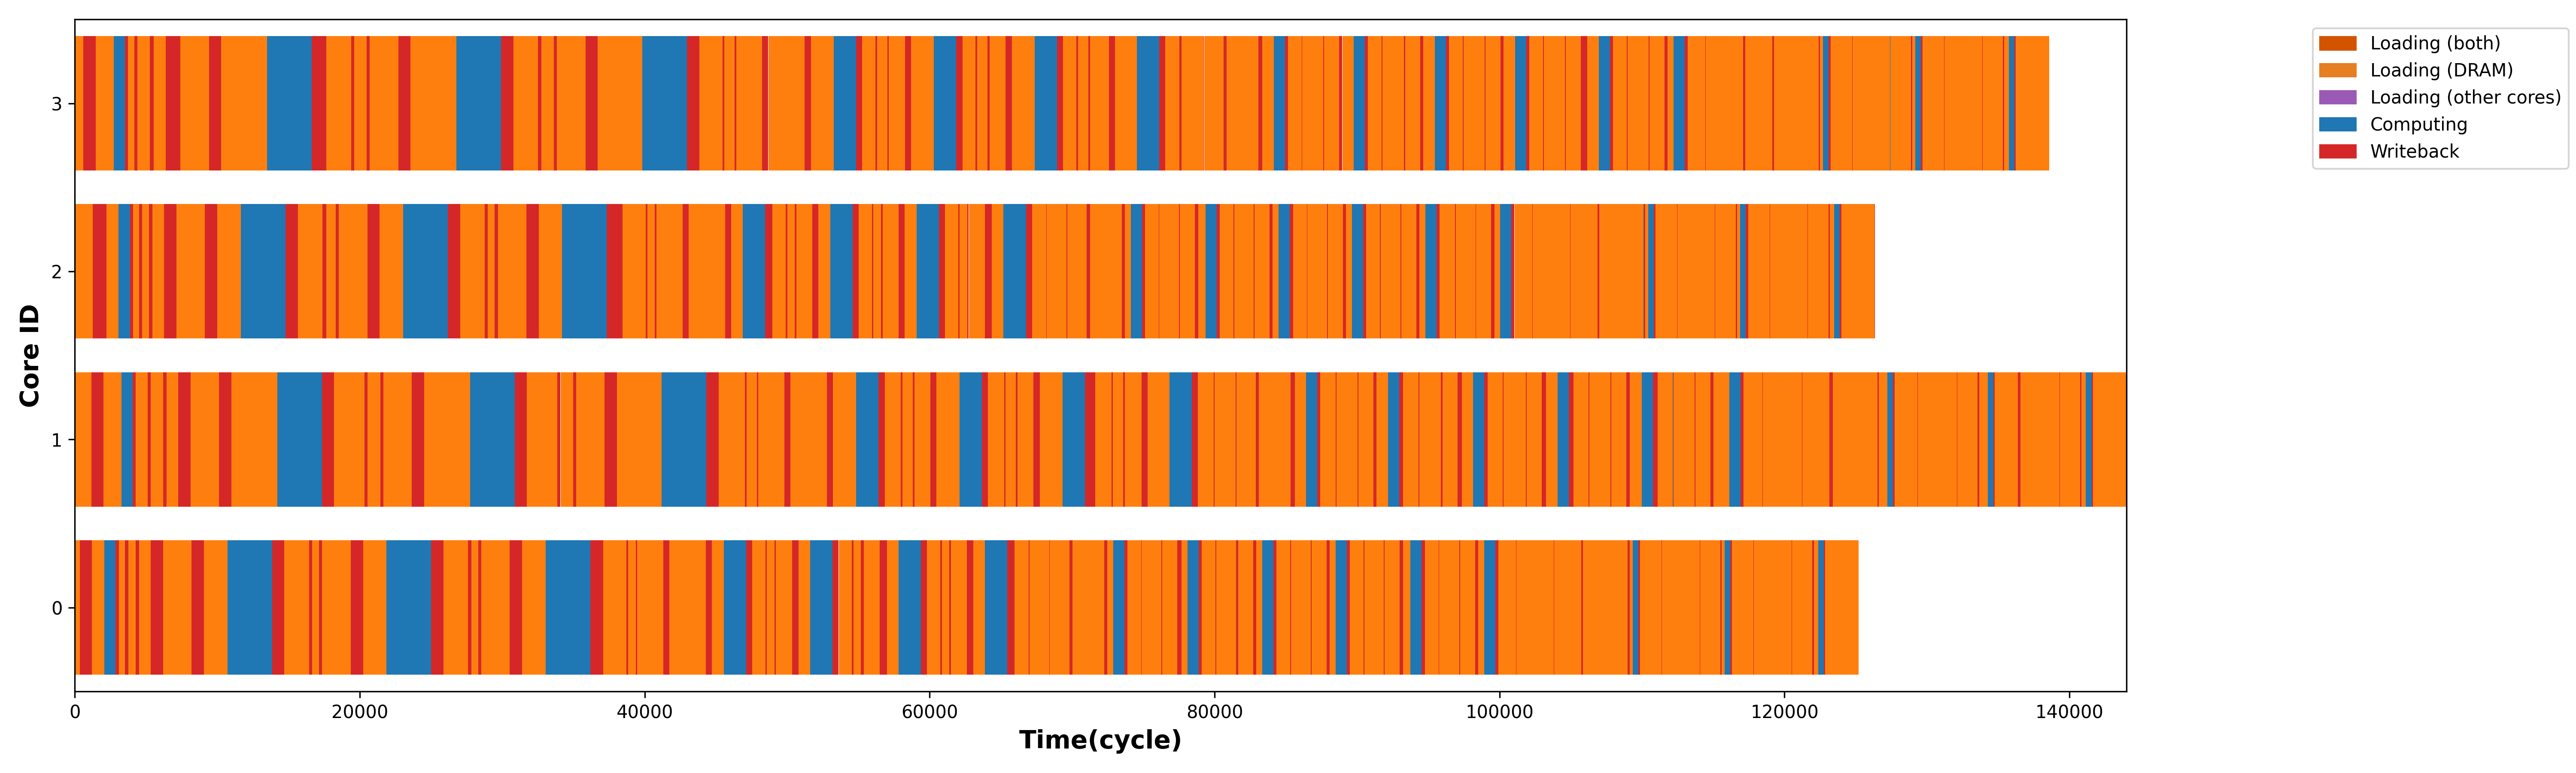
\includegraphics[width=\linewidth]{Figures/c5_gantt_hbm_optimized.png}
  \caption{HBM 优化甘特图}
  \label{fig:c5_gantt_hbm}
\end{figure}

残留瓶颈分析  虽然 HBM 的峰值 DRAM 带宽达到 \SI{128}{GB/s}（\SI{5120}{B/cycle}），远超加载数据所需，但加载阶段仍占各核活跃时间的约 60\%。对 288 个工作负载的逐项分析表明：92\% 的工作负载的加载时间受 SRAM 写端口带宽限制（\SI{256}{B/cycle}），而非 DRAM 响应延迟。具体而言，DRAM 数据到达核后必须按 SRAM 写带宽逐周期写入片上存储。当 DRAM 带宽远超 SRAM 写入速率时，后者成为新的瓶颈。这一“片上带宽墙”现象在高带宽外部存储配合传统窄端口 SRAM 时普遍存在。

第二轮模拟在 HBM 升级后将瓶颈从 DRAM 带宽迁移到了 SRAM 写端口，其中 92\% 的工作负载受 \SI{256}{B/cycle} SRAM 写带宽限制，第三轮即针对这一新瓶颈再做硬件改动，在 HBM 配置基础上将 SRAM 读写带宽从 \SI{256}{B/cycle} 提升至 \SI{1024}{B/cycle}，对应于在硬件设计上加宽 SRAM 读写端口或采用多 Bank 并行访问，其余参数（核微架构、NoC、DRAM）保持不变，重新运行模拟以验证三阶段是否趋于平衡。

实验结果方面，表\ref{tab:c5_sram_stats}给出 HBM + SRAM \SI{1024}{B/cycle} 配置下的模拟统计。

\begin{table}[H]
  \centering
  \caption{HBM + 宽 SRAM 模拟每核统计表}
  \label{tab:c5_sram_stats}
  \small
  \begin{tabular*}{\textwidth}{@{\extracolsep{\fill}}crrrrc}
    \toprule
    核 & IDLE & LOADING & COMPUTING & WRITEBACK & Workloads \\
    \midrule
    0  & 0      & 28,374  & 22,352  & 8,589   & 72 \\
    1  & 0      & 31,058  & 22,352  & 8,668   & 72 \\
    2  & 0      & 28,853  & 22,352  & 10,588  & 72 \\
    3  & 0      & 30,766  & 22,352  & 9,429   & 72 \\
    \midrule
    总计/最大 & --- & 119,051 & 89,408 & 37,274 & 288 \\
    \bottomrule
  \end{tabular*}
\end{table}

总周期降至 62,818，较 HBM（SRAM 256）再降 56.4\%，较 DDR4 基线降 73.7\%。LOADING\allowbreak /COMPUTING \allowbreak 比值从 4.1 降至 1.3，计算阶段占瓶颈核活跃时间的比例从 15.6\% 升至 35.7\%，系统从严重存储受限逐步趋向计算与存储的平衡。图\ref{fig:c5_hotspot_sram}的热力图显示，COMPUTING 占比升至 36\%--38\%，LOADING 降至 47\%--50\%，三阶段占比趋于均衡。图\ref{fig:c5_gantt_sram}的甘特图中，计算段（蓝色）面积明显增大，加载与写回段均大幅缩短。

\begin{figure}[H]
  \centering
  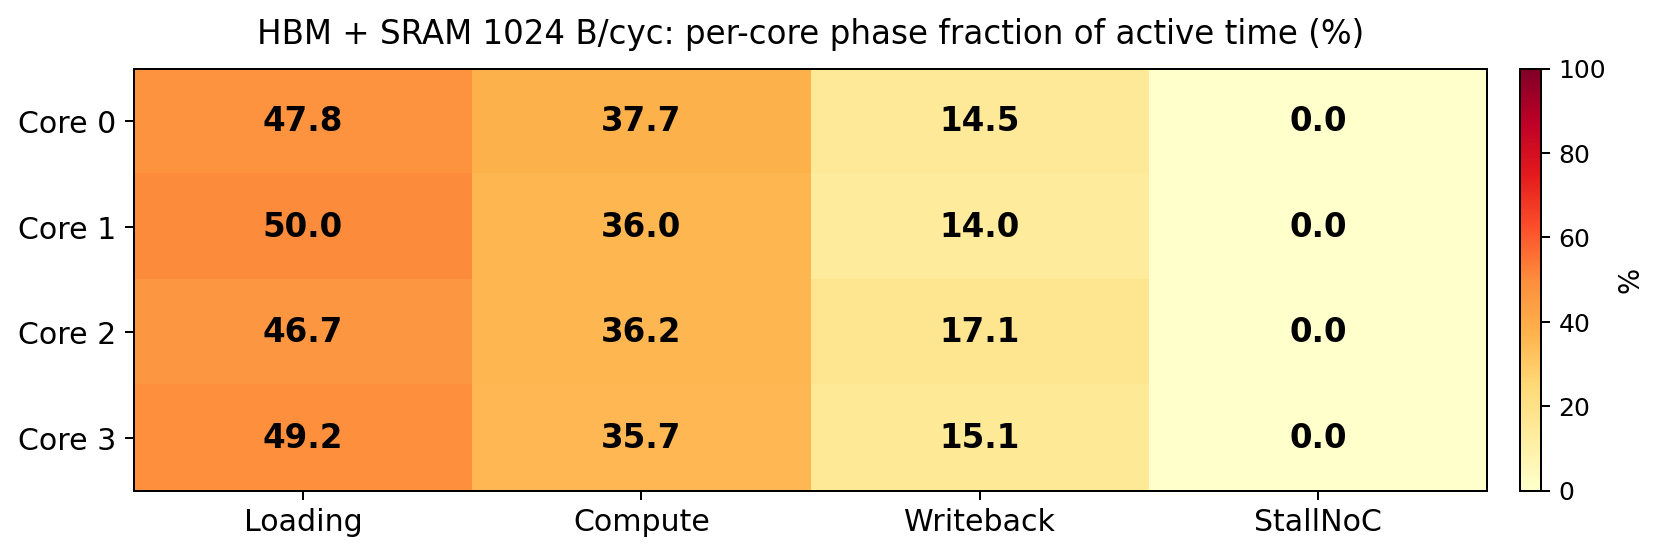
\includegraphics[width=0.88\linewidth]{Figures/c5_hotspot_hbm_sram1024.png}
  \caption{HBM + 宽 SRAM 各核阶段占比热力图}
  \label{fig:c5_hotspot_sram}
\end{figure}



\begin{figure}[H]
  \centering
  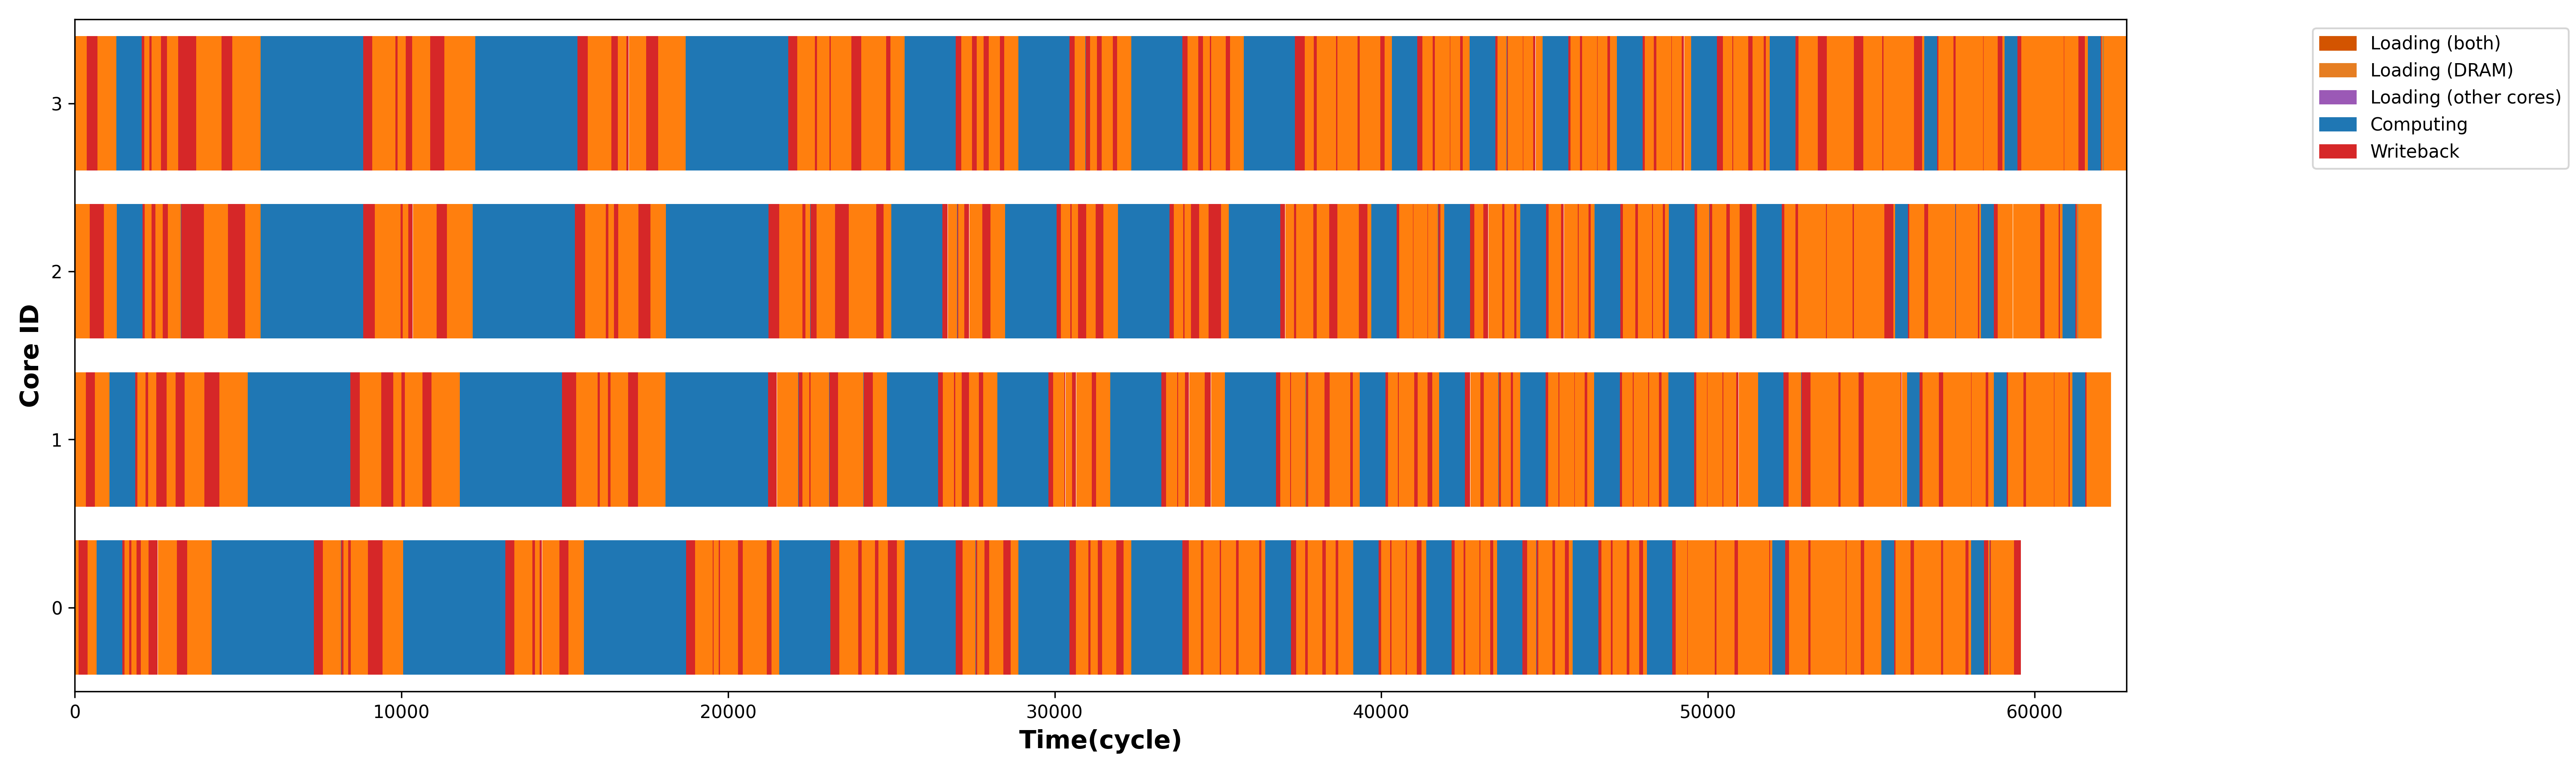
\includegraphics[width=\linewidth]{Figures/c5_gantt_hbm_sram1024.png}
  \caption{HBM + 宽 SRAM 甘特图}
  \label{fig:c5_gantt_sram}
\end{figure}

表\ref{tab:c5_comparison}汇总三组配置的关键指标，展示了优化路径的完整效果。

\begin{table}[H]
  \centering
  \caption{三组配置模拟结果对比表}
  \label{tab:c5_comparison}
  \small
  \begin{tabular*}{\textwidth}{@{\extracolsep{\fill}}lrrrc}
    \toprule
    指标 & DDR4 基线 & HBM 优化 & HBM+宽SRAM & 总改善 \\
    \midrule
    总周期            & 238,803   & 144,000  & 62,818   & $-$73.7\% \\
    相对DDR4加速比    & 1.00$\times$ & 1.66$\times$ & 3.80$\times$ & --- \\
    LOADING 总周期    & 592,071   & 370,183  & 119,051  & $-$79.9\% \\
    WRITEBACK 总周期  & 252,209   & 73,431   & 37,274   & $-$85.2\% \\
    COMPUTING 总周期  & 89,408    & 89,408   & 89,408   & 0\% \\
    LOADING/COMPUTING & 6.62       & 4.14      & 1.33      & --- \\
    瓶颈核计算占比    & 9.4\%      & 15.6\%    & 35.7\%    & --- \\
    DRAM 峰值带宽     & \SI{19.2}{GB/s} & \SI{128}{GB/s} & \SI{128}{GB/s} & --- \\
    SRAM 写带宽       & \SI{256}{B/cy}  & \SI{256}{B/cy} & \SI{1024}{B/cy} & --- \\
    \bottomrule
  \end{tabular*}
\end{table}

综上，沿"DDR4 → HBM → HBM + 宽 SRAM"三轮递进，瓶颈先后从 DRAM 读写带宽迁移至片上 SRAM 写端口、再迁移至计算单元，总周期由 238,803 降至 62,818（相对基线 3.80 倍），LOADING/COMPUTING 比由 6.6 降至 1.3，计算周期始终保持 22,352 cycles 不变；这一"逐级暴露新瓶颈—针对性优化—再次模拟"的迭代过程，揭示了高带宽外部存储下"片上带宽墙"现象的存在，也验证了模拟器在多核存储子系统设计空间探索中的实用价值。

\xsubsection{实验结论}{Experimental Conclusions}
\label{subsec:c5_bottleneck_overall}

综合 5.2.1 节单核与 5.2.2 节多核两组实验，可以从归因方法、瓶颈现象与设计启示三个角度给出整体结论。

本节所构建的"分解口径 + 按核可视化"归因框架在单核与多核两种规模下保持了一致的口径，将端到端时间严格拆分为计算、片上网络背压与访存等待三类周期，并同时支持全局占比汇总与按核空间分布展示。该框架在 5.2.1 节用于解释单核 ResNet 端到端时间的构成，又在 5.2.2 节用作三轮递进模拟中"前一轮瓶颈结论触发下一轮硬件改动"的判据，从而证明它具备跨规模、跨配置的通用归因能力，可作为后续设计空间探索的标准分析工具。

进一步对比单核与多核场景，可以发现瓶颈的相对地位差异显著。单核 ResNet34/50 上计算占比约 77\%--81\%，访存占比约 19\%--23\%，NoC 背压恒为 0，即使模型加深至 ResNet50，访存占比的上升也未改变"计算主导"的总体格局；一旦扩展到 4 核、ResNet50、DDR4 单通道的多核存储受限场景，访存等待则跃升为主导阶段，LOADING\allowbreak /COMPUTING \allowbreak 比可达 6.6，且仅靠升级 DRAM（DDR4 → HBM）无法消除，必须配合加宽 SRAM 端口才能将该比值压回 1.3 量级。这表明从单核到多核的扩展并非简单的算力线性叠加，而会触发外部带宽与片上供数路径的连锁瓶颈，单一维度的硬件升级往往只是完成"瓶颈迁移"而非"瓶颈消除"。

由此可对未来神经网络芯片在算力—存储平衡上的设计提炼三点参考。其一，"片外带宽—片上端口—计算阵列"应作为整体协同的三层资源进行联合优化，单独提升任一层都可能因相邻层成为新瓶颈而损失收益，5.2.2 节中 HBM 升级后 SRAM 写端口反成限速环节即为典型案例；其二，访存与计算的相对占比是判断系统是否处于"计算受限/带宽受限/片上供数受限"状态的可解释指标，建议在芯片早期架构探索中即以该指标作为权衡片上 SRAM 容量、端口宽度与外部 DRAM 配置的依据；其三，本文模拟器在迭代式硬件改动中能够保持各子系统贡献的可分离性（如 5.2.2 节三轮中各核计算时长恒为 22,352 cycles），这一性质使其能够准确反映"是哪一类硬件改动带来了多少收益"，为多核神经网络芯片的设计决策提供了定量证据。上述结论将作为 5.3 节多核吞吐量设计空间探索实验中各项参数选择（如 HBM 四通道 + \SI{1024}{B/cycle} SRAM 端口）的依据。

\xsection{多核吞吐量设计空间探索实验}{Design-Space Exploration Experiment for Multi-core Throughput}
\label{sec:c5_dse}

在实际推理部署中，吞吐量受单核算力、核数规模、片上存储与 die 面积等多因素共同约束。本节沿单核算力（MAC 规模）、核数扩展与批量三个维度展开设计空间探索。所有实验均采用 ResNet50 网络、HBM 四通道 DRAM 与 \SI{1024}{B/cycle} SRAM 带宽（5.2.2~节确定的最优存储配置），并使用高保真后端（BookSim2 + Ramulator2）。后续 caption 中不再重复这些公共参数，仅在正文中说明每组实验所变动的维度与取值。

\xsubsection{单核算力扩展实验}{Single-core MAC Scaling Experiment}

在 4 核配置下，将单核乘法累加单元数从 256 扫描至 512 和 1024，对批量为 1 和批量为 4 各运行一组模拟。

实验结果方面，表\ref{tab:c5_mac_sweep}给出 MAC 扫描结果。

\begin{table}[H]
  \centering
  \caption{MAC 规模扫描表}
  \label{tab:c5_mac_sweep}
  \small
  \begin{tabular*}{\textwidth}{@{\extracolsep{\fill}}ccrrrrc}
    \toprule
    MAC & 批量 & 总周期 & LOADING & COMPUTING & WRITEBACK & 计算占比 \\
    \midrule
    256  & 1 & 62,775  & 119,210 & 89,408  & 36,944  & 35.8\% \\
    512  & 1 & 62,778  & 119,220 & 89,408  & 36,946  & 35.8\% \\
    1024 & 1 & 62,776  & 119,223 & 89,408  & 36,935  & 35.8\% \\
    \midrule
    256  & 4 & 258,289 & 508,269 & 357,632 & 153,289 & 34.8\% \\
    512  & 4 & 258,289 & 508,269 & 357,632 & 153,289 & 34.8\% \\
    1024 & 4 & 257,969 & 510,067 & 357,632 & 153,290 & 34.8\% \\
    \bottomrule
  \end{tabular*}
\end{table}

三种 MAC 规模下的总周期几乎无差异（批量为 1 时均约 62,778，批量为 4 时均约 258,000），且 COMPUTING 总周期完全一致。这一看似反直觉的结果源于当前负载的特征：Gemini 编译器生成的 IR 中，288 个工作负载（批量为 1 时）有 75\% 的工作负载计算量极小（compute\_cycles $\leq$ 1），真正有显著计算的仅为 residual 层。即使将 MAC 翻四倍，瓶颈核的活跃时间仍由 LOADING 主导（L/C $\approx$ 1.33），计算缩减对总周期的贡献被淹没。结论：在当前存储配置下，系统处于存储受限状态，单纯提升单核算力无法提高吞吐量。

\xsubsection{核数扩展实验}{Core-count Scaling Experiment}

固定单核乘加器单元数量为 512，将核数从 4 核扩展至 16 核与 64 核。每种核数的 IR 由 Gemini 编译器针对对应拓扑重新生成。

实验结果方面，表\ref{tab:c5_core_sweep}给出核数扩展结果。

\begin{table}[H]
  \centering
  \caption{核数扩展实验结果表}
  \label{tab:c5_core_sweep}
  \small
  \begin{tabular*}{\textwidth}{@{\extracolsep{\fill}}lcrrrrc}
    \toprule
    拓扑 & 批量 & 总周期 & L/C & 计算占比 & Workloads & 状态 \\
    \midrule
    4 核 & 1 & 62,781   & 1.33  & 35.8\% &  288 & 完成 \\
    16 核 & 1 & 60,839   & 5.61  & 9.2\%  & 1136 & 完成 \\
    64 核 & 1 & ---       & ---   & ---    & 4544 & 死锁 \\
    \midrule
    4 核 & 4 & 257,827  & 1.42  & 34.8\% & 1152 & 完成 \\
    16 核 & 4 & 296,297  & 6.95  & 7.6\%  & 4544 & 完成 \\
    \bottomrule
  \end{tabular*}
\end{table}

对实验结果的分析如下：（1）核数由 4 扩展到 16：总周期几乎不降。批量为 1 时从 62,781 降至 60,839（仅 $-$3.1\%），批量为 4 时反而从 257,827 升至 296,297（$+$14.9\%）。原因在于：核数增加后工作负载被分散到更多核（从 288 增至 1136），但 16 核共享同一 DRAM 子系统导致读写竞争加剧，LOADING 与 WRITEBACK 剧增。L/C 从 1.33 升至 5.61（批量为 1 时）和从 1.42 升至 6.95（批量为 4 时），系统从接近均衡退回到严重存储受限。（2）64 核死锁。64 核配置下模拟无法完成：99.3\% 的工作负载完成后，剩余 30 个工作负载的 15 个核陷入互等状态。这是因为 ResNet50 的层级结构（约 72 个 unique 层）无法均匀分布到 64 核，Gemini 编译器生成的 IR 中大量核的工作负载极少，导致复杂的依赖链形成环路。结论：核数不宜超过负载的并行度上限。

图\ref{fig:c5_dse_4x4_b1}给出 16 核的端到端甘特图，LOADING 与 WRITEBACK 段占据绝大部分时间线，DRAM 争用严重。图\ref{fig:c5_hotspot_4x4_b1}进一步以热力图形式展示各核阶段占活跃时间的比例：全部核心的 LOADING 占比在 50\%--55\%、WRITEBACK 在 36\%--41\%，COMPUTING 仅约 9.3\%--9.5\%，与 5.2.2 节 DDR4 基线（4 核）的 9\%--10\% 接近，表明核数扩大 4 倍后系统从接近均衡退回到严重存储受限。

\begin{figure}[H]
  \centering
  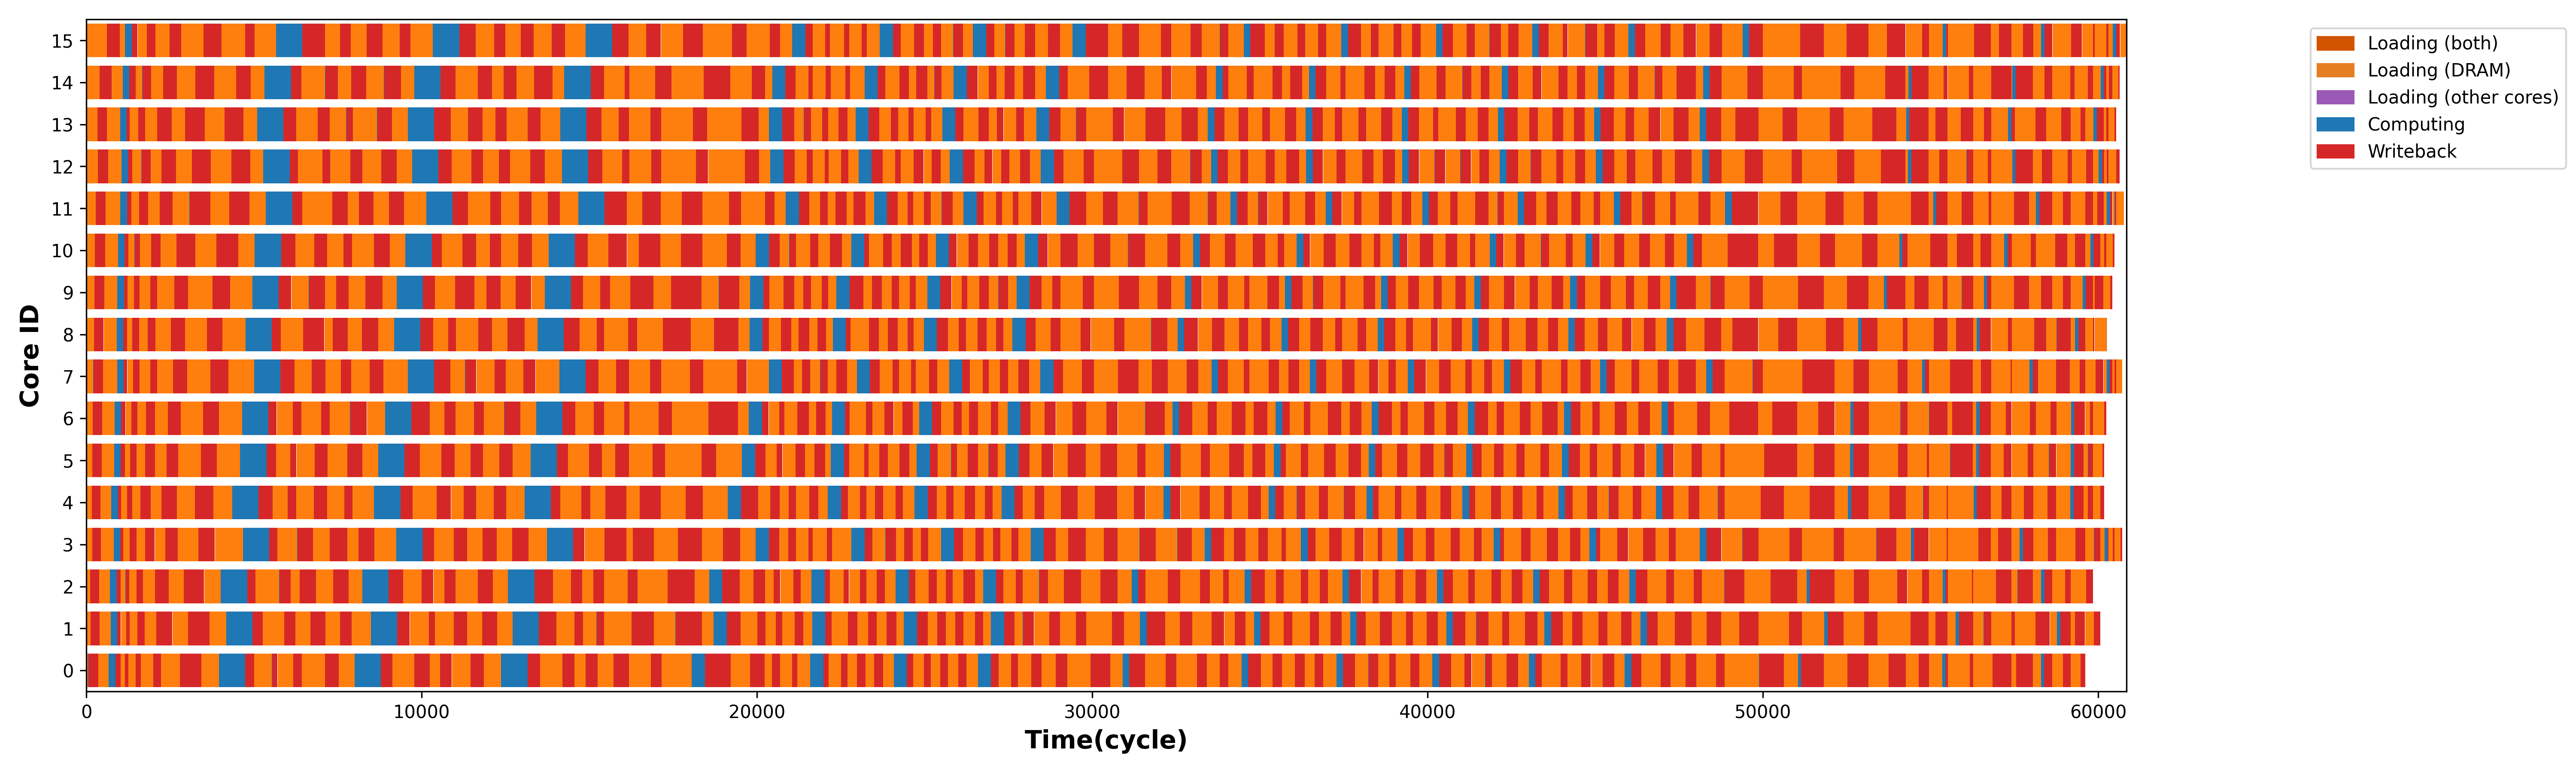
\includegraphics[width=\linewidth]{Figures/c5_dse_4x4_b1.png}
  \caption{16 核甘特图}
  \label{fig:c5_dse_4x4_b1}
\end{figure}

\begin{figure}[H]
  \centering
  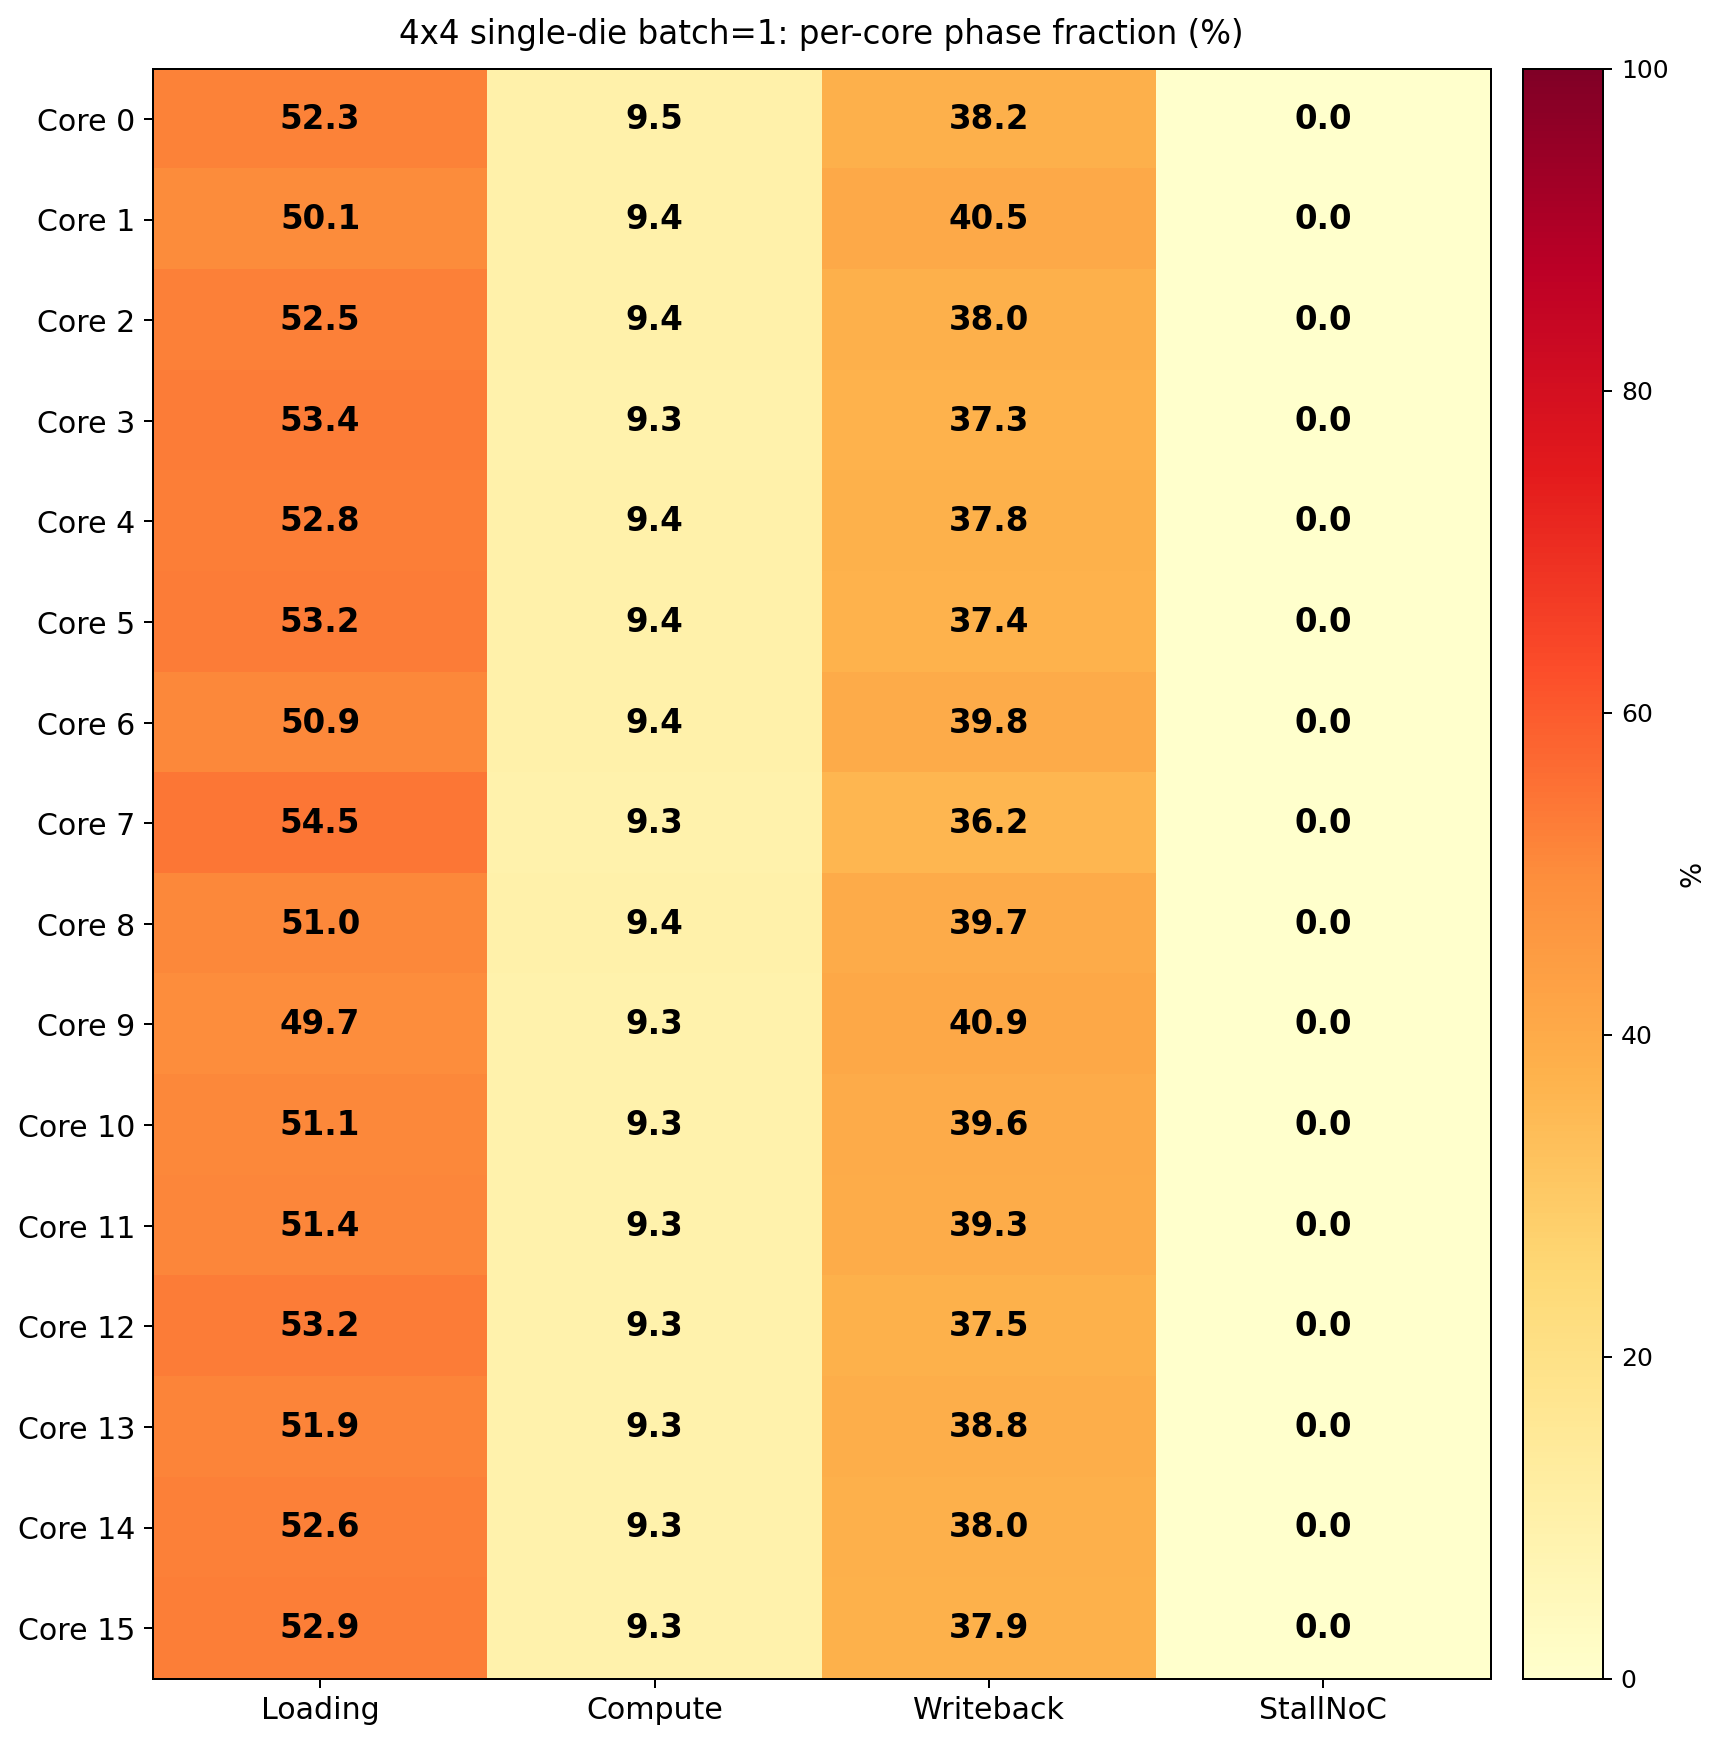
\includegraphics[width=0.88\linewidth]{Figures/c5_hotspot_4x4_b1.png}
  \caption{16 核各阶段占比热力图}
  \label{fig:c5_hotspot_4x4_b1}
\end{figure}

\xsubsection{批量扩展实验}{Batch Scaling Experiment}

在推理部署中，增大批量可以提高数据复用率与吞吐量。表\ref{tab:c5_batch}对比批量为 1 与批量为 4 在不同核数配置下的吞吐量。吞吐量定义为：
\begin{equation}
  \text{Throughput} = \frac{\text{Batch}}{\text{Total\_cycles}}\label{eqn:c5:throughput}
\end{equation}
式中：$\text{Throughput}$ 为单位周期完成的推理数。$\text{Batch}$ 为一次推理处理的样本数。$\text{Total\_cycles}$ 为完成该 Batch 推理所用的总仿真周期数。

\begin{table}[H]
  \centering
  \caption{批量扩展效率表}
  \label{tab:c5_batch}
  \small
  \begin{tabular*}{\textwidth}{@{\extracolsep{\fill}}lcrrrc}
    \toprule
    拓扑 & 批量 & 总周期 & 吞吐量（$\times 10^{-5}$/cyc） & 相对批量为 1 加速 & 效率 \\
    \midrule
    4 核 & 1 & 62,781  & 1.593 & ---     & --- \\
    4 核 & 4 & 257,827 & 1.551 & 0.97$\times$ & 24.3\% \\
    \midrule
    16 核 & 1 & 60,839  & 1.644 & ---     & --- \\
    16 核 & 4 & 296,297 & 1.350 & 0.82$\times$ & 20.5\% \\
    \bottomrule
  \end{tabular*}
\end{table}

批量从 1 增至 4 时，总周期增长约 4.1 倍（4 核）到 4.9 倍（16 核），均超过批量本身的 4 倍，导致吞吐量反而略降。批量扩展效率（= 批量为 4 时吞吐量 / 批量为 1 时吞吐量 / 4）仅约 24\%。这是因为在当前存储受限配置下，增大批量线性增加了 DRAM 读写数据量，但 DRAM 带宽并未同步扩展，导致存储争用超线性增长。

\xsubsection{实验结论}{Experimental Conclusions}

多核吞吐量设计空间探索实验的 12 组实验对比分析结论如下：（1）存储受限状态下，提升算力无效。当 LOADING/COMPUTING $>$ 1 时，系统为存储受限，增加 MAC 单元对吞吐量无贡献。设计者应优先解决 DRAM 带宽或 SRAM 端口带宽瓶颈，再考虑计算资源投入。（2）核数扩展存在明确上限。核数由 4 扩展到 16 时，在批量为 1 时仅提升 3\%，在批量为 4 时反而退步 15\%，64 核 直接死锁。核数必须与负载的并行度匹配：ResNet50 的有效并行度约 4--16 核，超过此范围后 DRAM 争用与调度依赖冲突主导性能。（3）批量扩展效率受限于存储带宽。批量为 4 相对批量为 1 的吞吐量效率仅约 24\%，说明在存储受限系统中批量扩展的收益远不及理想的线性关系，提升 DRAM 通道数或采用更高带宽的 HBM2E/HBM3 可望改善批量扩展效率。（4）模拟器对神经网络芯片设计的价值。本节实验覆盖了 12 种配置组合，每次模拟耗时 3--60 分钟，这一效率使得在流片前对核数、算力、存储带宽等关键参数进行快速定界成为可能。

\xsection{本章小结}{Chapter Summary}

本章围绕模拟器的可信性与实用价值组织了四组系统性实验。首先在双核与单核可控微基准上，通过片上网络同步实验、内存同步实验与模拟器精度验证实验，分别验证了核间依赖的因果一致性、DRAM 请求/响应闭环的正确性，以及在统一调度与高保真后端下与 Synopsys ZeBu 硬件模拟在 ResNet34、ResNet50 等真实负载上总周期相对误差控制在 $\pm$5.2\% 以内。其次在单核 ResNet 负载上提出基于计算、NoC 背压与访存等待的阶段占比分解口径，并辅以热点核与阶段占比的可视化，从全局占比与按核分布两个层面给出可解释的瓶颈归因。继而在四核测试芯片配置下围绕同一 ResNet50 负载，展示了从 DDR4 单通道基线到 HBM 四通道、再到加宽 SRAM 端口的逐级优化过程，将总周期从 238\,803 降至 62\,818（3.80 倍加速），并清晰呈现了瓶颈从片外带宽迁移到片上供数的迁移轨迹。最后沿单核算力、核数与批量三个维度开展 12 组设计空间探索实验，定量揭示了存储受限状态下提升算力无效、核数扩展存在并行度上限、批量扩展效率受存储带宽制约等系统级权衡。综合本章实验，本文模拟器在精度、瓶颈归因与多维设计空间探索能力三方面均得到了系统性验证，为流片前的多核神经网络芯片架构定界提供了可信、可解释、可重复使用的评估平台。
